\section{Zielsetzung}
Das Ziel dieses Versuches ist die Bestimmung der Anregungsenergie $W$ sowie der charakteristischen Relaxationszeit $\tau_0$ des dotierten Ionenkristalls Kaliumbromid.

\section{Theorie}
In diesem Versuch wird eine Kaliumbromidprobe untersucht.
Kaliumbromid ist ein Ionenkristall, welcher sich aus positiv geladenen Kaliumatomen und negativ geladenen Bromidatomen zusammensetzt.
Aufgrund der elektrostatischen Anziehungen gehen die Atome eine Ionenbindung ein, sodass sich eine, wie in Abbildung \ref{fig:tfig1} dargestellte, Kristallstruktur ergibt.

Durch Dotierung mit einem mehrwertigen Atom, wie zum Beispiel $\text{Sr}^{++}$, wird ein Ladungsüberschuss erzeugt, welcher aufgrund der notwendigen Ladungsneutralität des Kristalls durch eine Leerstelle ausgeglichen wird.
Diese Leerstelle befindet sich an dem Gitterplatz eines Kations und bildet zusammen mit dem Donatoratom einen permanten Dipol $\vec{P}$ im Kristall.
Wie in Abbildung \ref{fig:tfig2} zu sehen ist, sind aufgrund der Gitterstruktur des Kristalls nur diskrete Ausrichtungen des Dipols möglich.
Wegen der statistischen Verteilung der Dipolachsen, verschwindet das Gesamtdipolmoment des Kristalls.

\begin{figure}[H]
    \begin{subfigure}{0.48\textwidth}
    \centering
    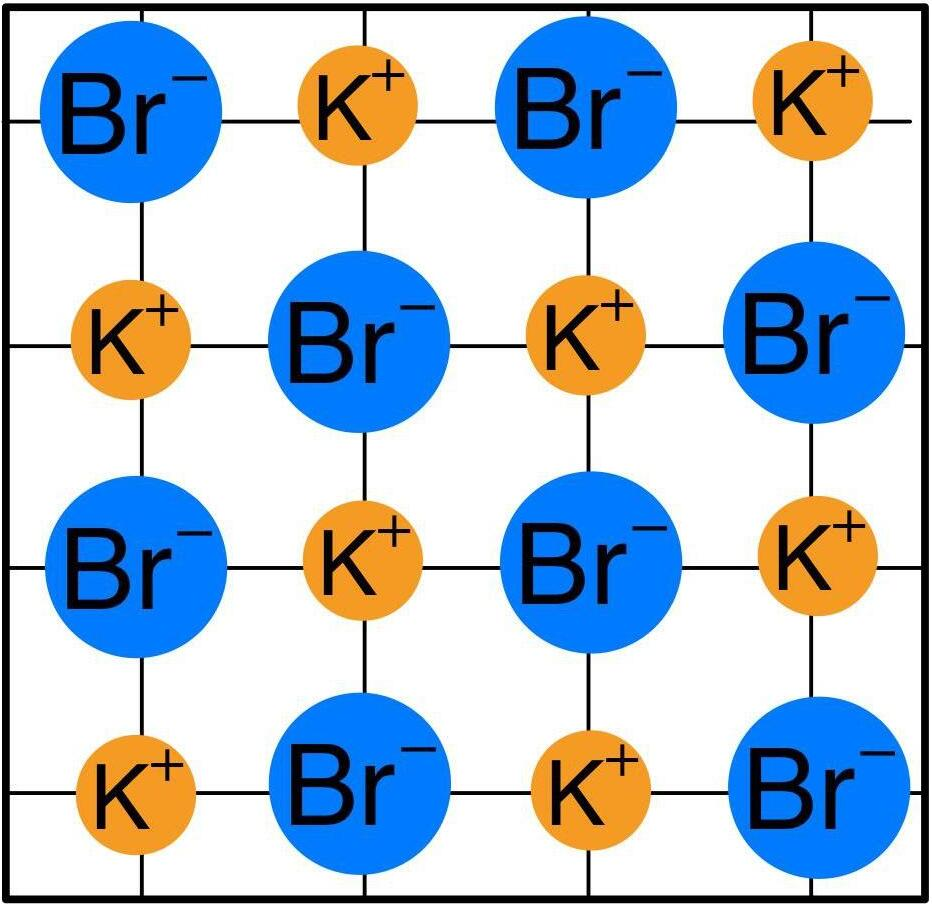
\includegraphics[width=0.85\linewidth]{figs/Kaliumbromid.jpg}
    \caption{Schematische Darstellung des Kristallgitters von Kaliumbromid.}
    \label{fig:tfig1}
    \end{subfigure}
    \begin{subfigure}{0.48\textwidth}
    \centering
    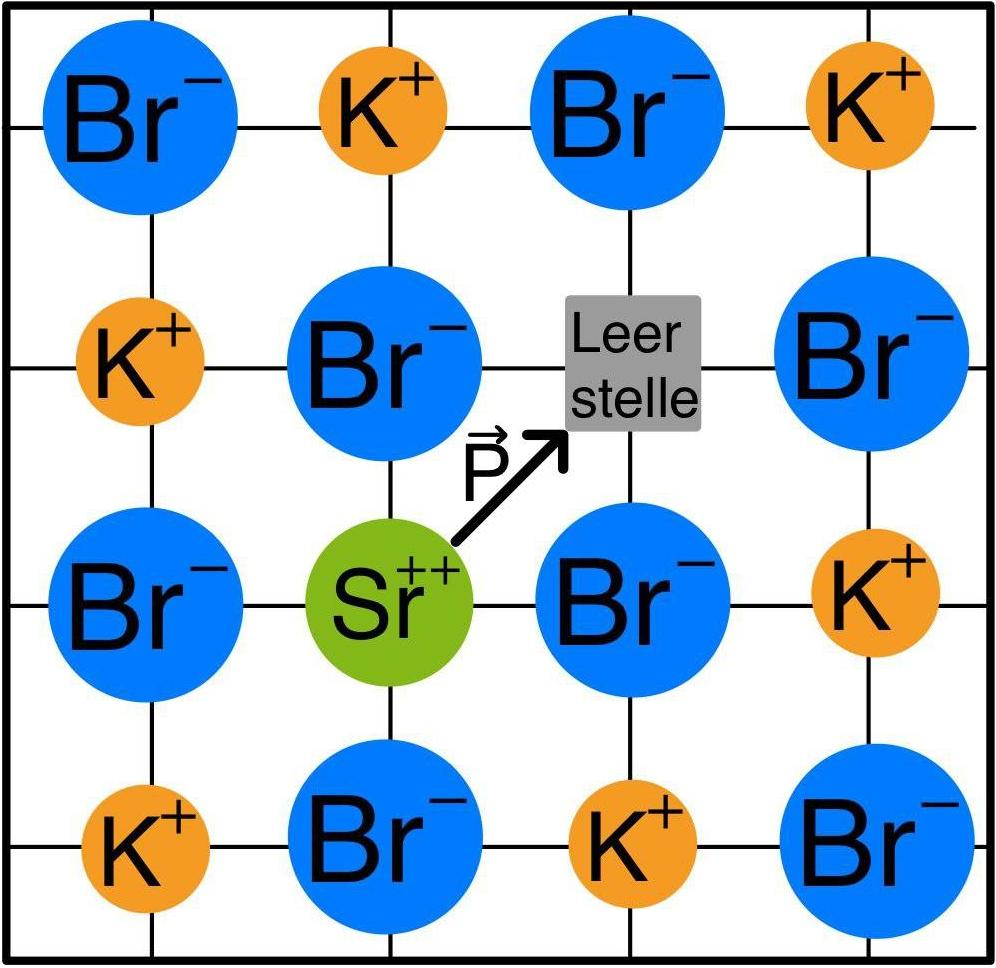
\includegraphics[width=0.85\linewidth]{figs/DipolKBr.jpg}
    \caption{Erzeugung eines Dipols im Ionenkristall durch Dotierung mit einem $\text{Sr}^{++}$-Atom.}
    \label{fig:tfig2}
    \end{subfigure}
    \caption{Darstellung des Ionenkristalls Kaliumbromid ohne und mit Dotierung durch ein Strontium Atom.}
\end{figure}

Bei Temperaturen unter $500°\symup{C}$ können sich nur die Leerstellen im Kristall bewegen, sodass die Ausrichtung eines Dipols nur durch Leerstellendiffusion geändert werden kann.
Um die Position einer Leerstelle zu ändern, muss eine gewissen Potentialschwelle überwunden werden.
Folglich ist für die Drehung eines Dipols eine materialspezifische Aktivierungsenergie $W$ erforderlich.
Nach der Boltzmann-Statistik ist der Anteil ${a=\exp(-\frac{W}{kT})}$ aller Dipole in der Lage die Aktivierungsenergie aufgrund ihrer thermischen Anregung aufzubringen.
Die temperaturabhängige Relaxationszeit
\begin{equation}\label{eq:relax}
  \tau(T)=\tau_0\exp\left( \frac{W}{kT}\right )
\end{equation}
ist die mittlere Zeit zwischen zwei Umorientierungen.
Hierbei wird $\tau_0$ charakteristische Relaxationszeit genannt und entspricht dem Grenzwert der Relaxationszeit für sehr hohe Temperaturen $\tau_0 = \tau(T\rightarrow \infty)$.

Wird die Probe in ein elektrisches Feld gebracht, ist der Anteil der Dipole, die sich entlang der Feldlinien ausrichten, durch die Langevin Funktion
\begin{equation}\label{eq:Langevin}
    y = L(x) = \coth(x)-\frac{1}{x} \qquad \text{mit} \qquad x=\frac{pE}{kT}
\end{equation}
gegeben.
Hierzu muss die Bedingung erfüllt sein, dass die Zeit in dem elektrischen Feld groß gegenüber der Relaxationszeit der Dipole ist.
Für $pE \ll kT$ kann die Langevin-Funktion durch eine Taylorentwicklung um $x=0$ zu 
\begin{equation}\label{eq:Langevin2}
    y(T)=\frac{pE}{3kT}
\end{equation}
genähert werden.
Aufgrund des exponentiellen Zusammenhangs zwischen Relaxationszeit und Temperatur \eqref{eq:relax} lässt sich ein erzeugtes Dipolmoment des Kristalls einfrieren, indem dieser stark abgekühlt wird.
Dadurch steigt die Relaxationszeit exponentiell an, sodass die Dipole quasi nicht mehr in der Lage sind ihre Richtung zu ändern.
Beim erneuten Erwärmen des Kristalls kehren diese nach und nach in ihre statistisch verteilten Ausgangspositionen zurück, sodass aufgrund der zeitlichen Änderung des Dipolmoments ein Dipolstrom in Abhängigkeit der Temperatur beobachtet wird.
Anhand dieses sogenannten Depolarisationsstroms sollen im Folgenden die Aktivierungsenergie $W$ und die charakteristische Relaxationszeit $\tau_0$ abgeleitet werden.

\subsection*{Herleitung des Depolarisationsstroms über die Stromdichte}
Die Depolarisationsstromdichte setzt sich zusammen aus dem Anteil der ausgerichteten Dipole \eqref{eq:Langevin} bei einer Polarisationstemperatur $T_\text{p}$, dem Dipolmoment $p$ und der Relaxationsrate $\frac{\symup{d}N}{\symup{dt}}$ der Dipole pro Volumeneinheit
\begin{equation}\label{eq:stromdichte}
    j(T)=y(T_p)\,p\,\frac{\symup{d}N}{\symup{d}t} \stackrel{\eqref{eq:Langevin2}}{=} \frac{p^2 E}{3kT_p}\frac{\symup{d}N}{\symup{d}t} \, .
\end{equation}
Bei einer konstanten Heizrate $b = \frac{\symup{d}T}{\symup{d}t}$ lässt sich die Relaxaktionsrate aus der Relaxationszeit \eqref{eq:relax} zu
\begin{align}
    \frac{\symup{d}N}{\symup{d}t} & = -\frac{N}{\tau(T)}\notag \\
    \Leftrightarrow \quad N & = N_\text{p}\exp\left(-\int_{t_0}^t \frac{\symup{d}t'}{\tau(T)}\right)\notag \\
    & = N_\text{p}\exp\left(-\frac{1}{b}\int_{T_0}^T \frac{\symup{d}T'}{\tau(T')}\right)\label{eq:AnzN}
\end{align}
bestimmen.
Hierbei ist $N_\text{p}$ die Anzahl der ausgerichteten Dipole pro Volumeneinheit zum Zeitpunkt $t_0$ bei der Temperatur $T_0$.
Mit der Relaxationszeit \eqref{eq:relax} und der Anzahl der Dipole N \eqref{eq:AnzN} ergibt sich für die Depolarisationsstromdichte \eqref{eq:stromdichte} der Ausdruck
\begin{equation}\label{eq:stromdichte2}
    j(T)= \frac{p^2E}{3kT_\text{p}}\frac{N_\text{p}}{\tau_0}\exp\left(-\frac{1}{b\tau_0}\int_{T_0}^T \exp\left(-\frac{W}{kT'}\symup{d}T'\right) \right)\exp\left(-\frac{W}{kT}\right)\, .
\end{equation}
Zu Beginn des Depolarisationprozesses ist stets
\begin{equation*}
    \int_{T_0}^T \exp\left(-\frac{W}{kT}\symup{d}T' \right) \approx 0\, ,
\end{equation*}
sodass für die Depolarisationsstromdichte im Anfangsbereich die Näherung
\begin{equation}
    j(T)\approx    \frac{p^2 E}{3kT_\text{p}}\frac{N_\text{p}}{\tau_0}\exp\left(-\frac{W}{kT}\right)
    \label{eq:anlauf}
\end{equation}
gilt.
Aus dem Verlauf des Depolarisationsstroms zu Beginn des Erwärmungsprozesses kann also die Aktivierungsenergie $W$ abgeleitet werden.

\subsection*{Herleitungs des Depolarisationsstroms über den Polarisationsansatz}
Der Polarisationsansatz
\begin{equation*}
    \frac{\symup{d}P}{\symup{d}t}=-\frac{P(t)}{\tau(T(t))}
\end{equation*}
ermöglicht eine genauere Bestimmung der Aktivierungsenergie $W$, indem der gesamte Verlauf des Depolarisationsstroms betrachtet wird.
Hierbei beschreibt $P$ die Polarisation der Probe, welche dem Gesamtdipolmoment pro Volumeneinheit entspricht.
Die Änderung der Polarisation in eine Probe mit dem Querschnitt $F$ resultiert in einem messbaren Strom
\begin{equation}\label{eq:strom}
    i(t)=F\,\frac{\symup{d}P}{\symup{d}t} \, .
\end{equation}
Unter der Voraussetzung, dass die Erwärmung der Probe mit einer konstanten Heizrate erfolgt und somit $T\sim t$ ist, folgt durch Integration der Gleichung \eqref{eq:strom} für die Relaxationszeit
\begin{align}
    \tau(T)&= \frac{\int_T^\infty i(T')\symup{d}T'}{i(T)b}\\
    \stackrel{\eqref{eq:relax}}{\Leftrightarrow}\quad \frac{W}{kT} &= \ln \left(\frac{\int_T^\infty i(T')\symup{d}T'}{i(T)\tau_0 b}\right) \label{eq:integral}
\end{align}
In der Anwendung genügt es die obere Integrationgrenze durch einen Wert $T^*$ zu ersetzen, für welchen $i(T^*)\approx 0$ ist.

\subsection*{Bestimmung der charakteristischen Relaxationszeit aus dem Maximum des Depolarisationsstroms}
Die charakteristische Relaxationszeit $\tau_0$ wird aus der Lage des Maximums des Depolarisationsstroms abgeleitet.
Durch Differentiation der Depolarisationsstromdichte \eqref{eq:stromdichte2} ergibt sich der Zusammenhang zwischen Relaxationszeit und Temperatur zu
\begin{equation}
    \tau(T_\text{max})=\frac{k T_\text{max}^2}{bW} \,.
    \label{eq:tmax}
\end{equation}
Einsetzen des Wertepaares $(T_\text{max}, \tau(T_\text{max}))$ in Gleichung \eqref{eq:relax} liefert die charakteristische Relaxationszeit $\tau_0$.


